\chapter{Slovo Romana}
Titulní strana v~takové podobě, v~jaké se vám dostala, je navzdory veškeré projevené snaze velice chatrná a proto vám radím příliš nezasahovat do její stavby, neboť by to mohlo zcela rozhodit pozice všech objektů.
Primární snahou bylo dosáhnout její netečnosti vůči příliš dlouhým jménům (doc.
RNDr.
Jana Šťastně Vdaná, Ph.D.), názvům práce a názvům škol.

I~v~sekci Prohlášení zkuste držet svého kreativního ducha na uzdě, abyste jej vzápětí uplatnili v~celém následujícím textu.
Struktura textu by měla být zhruba následující:

\begin{enumerate}
\item[$\bullet$] úvod
\item teorie
\item metodika
\item výsledky
\item diskuze
\item[$\bullet$] závěr
\end{enumerate}
nicméně není pevně daná a spoustě prací sluší i tematičtější způsoby dělení informací.

\section{Plovoucí objekty}
Všechna čest Microsoftu za postupnou konverzi Wordu z~textového procesoru v~sázecím software.
Jedna z~mnoha vlastností nových verzí je možnost přidání titulku k~plovoucímu objektu, jako bývá obrázek či tabulka.

\begin{figure}[h]
  	\centering
 	
\includegraphics[width=200px]{img/final_doc.png}
 	\caption{Vás to nejspíše čeká taky.}
\end{figure}

\begin{table}[h]
  \centering
    \begin{tabular}{|l|l|}
    \hline
    Jednoduchá & tabulka \\ \hline
    o~& ničem \\
    \hline
    \end{tabular}
  \caption{Jak vidno, čísluje se separátně}
\end{table}

\begin{listedequation}[h]
$$L = - \frac{1}{4}F_{{\mu}v}F^{{\mu}v} + i \overline{\psi} \psi + \psi_i y_i \psi_j \phi + hc + |D_\mu\phi|^2 - V(\phi)$$
\caption{To je ale rovnice!}
\label{eq:hrnekeq}
\end{listedequation}

Vkládání popisků k~obrázkům a tabulkám lze zařídit poměrně snadno a intuitivně tlačítkem „Vložit titulek“ na kartě \It{Reference}.
U~rovnic se bohužel tento způsob uplatňuje jen velmi těžko, klasické vpravo zarovnané (1.1) lze pouze vykouzlit.
(Nápověda Microsoftu radí použít VBA makro, přívrženci Visual Basicu tedy nebudou mít problém.
Obávám se ale, že takových moc nebude.)

Využijte funkci „Vložit seznam obrázků“, která krom seznamu obrázků umí vkládat i seznam tabulek nebo rovnic.
Seznam obrázků v~práci být musí, i kdyby tam byl jen jeden obrázek.
Pro případ nejasnosti upřesňuji, že graf je považován za obrázek.

Co se dá naopak použít skvěle, jsou křížové odkazy.
Klepnutím na tlačítko „Křížový odkaz“ na kartě \It{Reference} mi umožní v~textu odkazovat na právě nějaký z~plovoucích objektů (či kapitolu, sekci, …) Proto nemám potíž zde uvést, že rovnice \autoref{eq:hrnekeq} odpovídá rovnici vyobrazené na hrnku na \autoref{fig:hrnek}, jen s~tím rozdílem, že na hrnku není formulována zcela správně.

\begin{figure}[h]
  	\centering
 	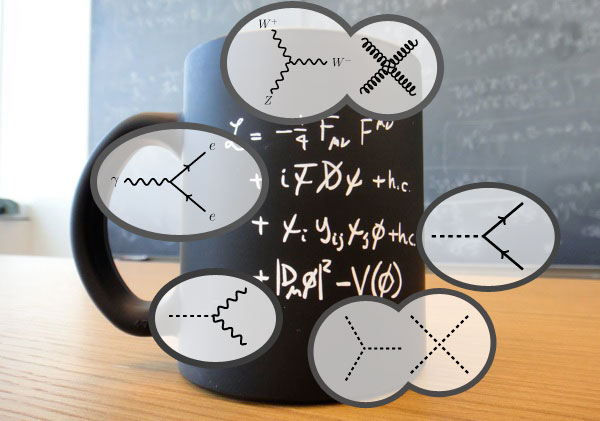
\includegraphics[width=\textwidth]{img/hrnek.jpg}
 	\caption{Hrneček ze Švýcarska}
 	\label{fig:hrnek}
\end{figure}

\section{Bibliografie}
Citovat je důležité (kruciální) a neméně důležité je citovat správně, a to v~ČR podle normy ČSN ISO 690 a ČSN ISO 690-2.
Důvod, proč ji tak mnoho lidí nedělá, je takový: Jedná se o~pěkně otravnou činnost\cite{citovani}.
To se však dá značně eliminovat použitím vhodného softwaru na správu a export citací.
Jaké máme možnosti?

Přímo českou normou se již dlouhou dobu zabývá projekt Citace.com umožňující zdarma získat toliko potřebné bibliografické záznamy.
Proces zkomfortňování šel až tak daleko, že si (např.) čtenáři registrovaní v~Moravské zemské knihovně (do 19 let vč.
zdarma) mohou nainstalovat do svého Wordu doplněk, který téměř vše zařídí za vás.

Pokud náhodou ještě nemáte a nemůžete mít účet v~Moravské zemské knihovně, nemusíte zoufat, i volně přístupná část nástrojů Citací.com má co nabídnout.
Na webu totiž můžete jednoduše vložit ISBN knihy nebo DOI (\It{Digital object identifier}) článku v~časopise a obratem vám bude vygenerována citace přesně podle normy, kterou můžete jednoduše zkopírovat do Wordu.
Číslování v~textu si však budete muset řešit sami.

Nicméně možnosti nekončí Citacemi.com, existuje celá řada dalších nástrojů (třeba EndNote).
Nebojte se požádat o~pomoc své školitele, sami si nejednou prošli stejným problémem a řešení s~velkou pravděpodobností našli.
Tak proč vynalézat kolo?

\subsection{Užitečné odkazy}
\begin{itemize}
    \item \url{http://www.citace.com}, \url{http://www.mzk.cz/}
	\item \url{http://www.boldis.cz/citace/citace1.pdf}
	\item \url{http://www.boldis.cz/citace/citace2.pdf}
	\item \url{https://sites.google.com/site/novaiso690/}
\end{itemize}

\section{Symboly, zkratky, slovníček}
Zkratky vysvětlujeme již při první zmínce v~textu, při jejich častějším výskytu může být praktické uvést ucelený seznam.
Totéž pak platí pro pojmy, které vysvětlujeme v~poznámce pod čarou\footnote{Poznámku pod čarou vložíme opět z~karty \It{Reference} tlačítkem \It{Vložit pozn.
pod čarou.}}: pokud jich je mnoho, vysázíme je i samostatně jako slovníček pojmů.

\section{Moudra závěrem}
Uvědomte si, že hlavním výstupem vaší roční činnosti nejsou data nebo zařízení, nýbrž právě odborný text, který má komisi SOČ ukázat, jak jste studované problematice porozuměli, jaký je váš vlastní přínos, jestli dokážete verbálně vystihnout vše podstatné a důležité.
\It{Formální a estetickou úpravou práce sdělujete komisi, jak moc vám záleží na tom, aby pro ně bylo čtení vaší práce příjemným či alespoň snesitelným zážitkem.}

Šablona je míněna jen jakýmsi odrazovým můstkem a nebojte, pořád na vás zbylo docela dost práce.
Bohužel víc, než jsem původně zamýšlel, protože sázení ve Wordu stále není žádný med a byla by jistě škoda ochudit vás o~četné nadávky na nesmyslnost jeho chování.
Všem počítačově zdatným jedincům pak doporučuji naučit se sazbu v~LaTeXu, je to dovednost, která se vám nikdy neztratí.

\begin{figure}[h]
  	\centering
 	
\includegraphics[width=\textwidth]{img/pulp.jpg}
 	\caption{Nejste v~tom sami.}
\end{figure}

Na závěr vám už poradím jen jedno: hledejte inspiraci.
Velmi dobře si pamatuji ten pocit, kdy sedíte nad prázdným dokumentem a přemýšlíte, co vlastně do té SOČky patří.
Kde začít? Co ještě zmínit a co už raději vynechat? Přitom máme všichni díky theses.cz na dosah stovky tisíc závěrečných prací starších kolegů z~vysokých škol.
Najděte si svůj vzor a jeďte podle něj, odborné posudky vedoucích a oponentů vám dokonce řeknou, co je správně a co nikoliv.

\vspace{\baselineskip}
\noindent Vědě zdar!

\vspace{\baselineskip}
\noindent \B{Roman Beránek} \\
\url{ischemy@gmail.com}
